% ============================================================
%  CudaNN: Training a CNN From Scratch Using CUDA
%  Shiraz University Report
% ============================================================
\documentclass[10pt,twocolumn,letterpaper]{article}

% ---- packages ----
\usepackage[utf8]{inputenc}
\usepackage[T1]{fontenc}
\usepackage[margin=2cm]{geometry}
\usepackage{graphicx}
\usepackage{amsmath,amssymb}
\usepackage{booktabs}
\usepackage{caption}
\usepackage{subcaption}
\usepackage{hyperref}
\usepackage{xcolor}
\usepackage{listings}
\usepackage{enumitem}
\usepackage{float}
\usepackage{fancyhdr}
\usepackage{titlesec}
\usepackage{tikz}
\usepackage{pgfplots}
\usepackage{pgfplotstable}
\usepackage{colortbl}
\usepackage{multirow}
\usepackage{array}

\pgfplotsset{compat=1.18}
\usetikzlibrary{shapes.geometric, arrows.meta, positioning, calc, patterns, decorations.pathreplacing}

% ---- color palette ----
\definecolor{shirazblue}{RGB}{0,75,135}
\definecolor{shirazgold}{RGB}{200,160,50}
\definecolor{shirazgray}{RGB}{100,100,100}
\definecolor{codeblue}{RGB}{0,80,160}
\definecolor{codegray}{RGB}{110,110,110}
\definecolor{codebg}{RGB}{245,245,245}
\definecolor{accentred}{RGB}{180,40,40}
\definecolor{accentgreen}{RGB}{30,130,76}
\definecolor{accentorange}{RGB}{220,130,30}
\definecolor{accentpurple}{RGB}{100,60,160}
\definecolor{lightblue}{RGB}{220,235,250}
\definecolor{tableheader}{RGB}{0,75,135}
\definecolor{tablerow1}{RGB}{240,245,250}
\definecolor{tablerow2}{RGB}{255,255,255}

% ---- listings style ----
\lstset{
  basicstyle=\ttfamily\scriptsize,
  keywordstyle=\color{codeblue}\bfseries,
  commentstyle=\color{codegray}\itshape,
  backgroundcolor=\color{codebg},
  frame=single, breaklines=true, captionpos=b,
  numbers=left, numberstyle=\tiny\color{codegray}, tabsize=2,
}

% ---- header / footer ----
\pagestyle{fancy}
\fancyhf{}
\fancyhead[L]{\small \textit{Multicore \& GPU Programming --- Fall 2025}}
\fancyhead[R]{\small \textit{Shiraz University}}
\fancyfoot[C]{\thepage}
\renewcommand{\headrulewidth}{0.4pt}

% ---- title formatting ----
\titleformat{\section}{\large\bfseries\color{shirazblue}}{\thesection.}{0.5em}{}[\vspace{-4pt}\textcolor{shirazblue}{\rule{\columnwidth}{0.5pt}}]
\titleformat{\subsection}{\normalsize\bfseries}{\thesubsection.}{0.5em}{}

% ---- hyperref setup ----
\hypersetup{colorlinks=true, linkcolor=shirazblue, citecolor=shirazblue, urlcolor=shirazblue}

% ---- custom table style ----
\newcommand{\tablehead}[1]{\textcolor{white}{\textbf{#1}}}
\newcolumntype{C}[1]{>{\centering\arraybackslash}p{#1}}

% ============================================================

\title{\LARGE\bfseries Training a Convolutional Neural Network
   From Scratch Using CUDA:
   Implementation, Profiling, and Bottleneck Analysis}

\author{Mehdi Khameedeh \qquad Salar Rahnama \\[6pt]
  \normalsize Supervisor: Dr.\ Farshad KhunJush \\[4pt]
  \normalsize Department of Computer Science and Engineering \\
  \normalsize Shiraz University \\[4pt]
  \normalsize Multicore \& GPU Programming, Fall 2025 \\[4pt]
  \small\color{shirazgray} February 2026}

\date{}

\begin{document}

\twocolumn[
  \maketitle
  \begin{@twocolumnfalse}
  \begin{abstract}
  \noindent We present \textbf{CudaNN}, a high-performance training platform for convolutional neural networks implemented entirely in CUDA~C++ from first principles, bypassing standard deep learning frameworks to expose the raw underlying hardware interaction.
  The system supports diverse architectures---LeNet, SimpleCNN, and MLP---across MNIST, CIFAR-10, and Synthetic datasets, featuring a hand-optimized stack: host-to-device streaming with double-buffered pinned memory, asynchronous checkpointing via background threads, log-synchronization reduction, and norm-logging throttling.
  We perform systematic profiling on an NVIDIA GeForce RTX~3050 Laptop GPU, revealing a critical \emph{latency-bound regime} for small-batch deep learning workloads.
  Our analysis demonstrates that on lightweight architectures, the dominant performance limiter is not arithmetic throughput but \emph{kernel-launch and synchronization overhead}: extremely low occupancy kernels ($\sim$1\% for bias gradients) and thousands of micro-scale device-to-host transfers ($\sim$18 bytes/call) create a control-bound environment where the GPU remains 85\% idle despite active kernel execution.
  This report provides a detailed case study in the systems-level challenges of bare-metal GPU programming, creating a clear distinction between compute-bound optimization (tiling, tensor cores) and latency-bound optimization (kernel fusion, launch minimization).

  \medskip
  \noindent\textbf{Keywords:} CUDA, GPU Profiling, Kernel Occupancy, Latency-Bound Execution, From-Scratch Training, Control Overhead
  \end{abstract}
  \vspace{16pt}
  \end{@twocolumnfalse}
]

% ============================================================
\section{Introduction}
\label{sec:intro}

Graphics Processing Units (GPUs) drive modern deep learning by providing massive parallelism through thousands of cores.
While frameworks like PyTorch and TensorFlow abstract away memory management and kernel dispatch, they often obscure the \emph{fine-grained interaction} between host orchestration and device execution.
For large models (e.g., Transformers), execution is compute-bound, utilizing the GPU's teraflops of throughput.
However, for smaller, experimental, or real-time workloads, the bottleneck often shifts to the \emph{control plane}---a regime where the overhead of launching kernels and synchronizing data outweighs the computation itself.

In this project, we accept the challenge of building a complete neural network training engine from scratch in CUDA~C++.
By managing every byte of memory and writing every kernel by hand, we expose the structural inefficiencies that usually remain hidden.
Our platform, \textbf{CudaNN}, serves as both a functional training system and a vehicle for systems-level performance analysis.

Our primary contribution is not just the implementation, but the \emph{characterization of the overhead-bound regime}.
We show that standard optimizations like asynchronous pipelining---which are critical for maximizing throughput on large workloads---can paradoxically degrade performance on lightweight models (e.g., MLP on Synthetic data) due to the added orchestration cost.
Through detailed profiling, we identify specific pathological patterns: \emph{micro-kernels} with $\sim$1\% occupancy that fail to saturate the GPU's massive parallelism, and \emph{synchronization thrashing} caused by frequent retrieval of scalar metrics (loss, accuracy) from device memory.

\paragraph{Key Contributions.}
\begin{enumerate}[nosep,leftmargin=*]
  \item \textbf{Bare-Metal Implementation:} A complete CUDA~C++ training stack with hand-written kernels for convolution, pooling, and backpropagation, managing raw pointers and explicit memory barriers.
  \item \textbf{Modular Optimization Stack:} A set of independently togglable optimizations targeting data transfer overlap, synchronization dampening, and memory reuse.
  \item \textbf{Bottleneck Analysis:} A quantitative dissection of performance limiters, identifying \emph{kernel launch overhead} and \emph{micro-transfers} as the primary bottlenecks for small-scale deep learning, contrasting sharply with the compute-bound nature of large-scale training.
\end{enumerate}

\paragraph{Organization.}
Section~\ref{sec:arch} describes the software architecture and CUDA kernel design.
Section~\ref{sec:optim} details each optimization and its expected impact.
Section~\ref{sec:setup} presents the experimental methodology.
Section~\ref{sec:results} analyzes training correctness, step times, memory overhead, and GPU utilization.
Section~\ref{sec:bottlenecks} provides a deep-dive into each bottleneck category.
Section~\ref{sec:discussion} discusses the structural implications.
Section~\ref{sec:conclusion} concludes.


% ============================================================
\section{System Architecture}
\label{sec:arch}

\subsection{High-Level Design}

CudaNN is composed of CPU-side orchestration modules and GPU-side compute modules, as shown in Figure~\ref{fig:sysarch}.

\begin{figure}[H]
\centering
\resizebox{\columnwidth}{!}{%
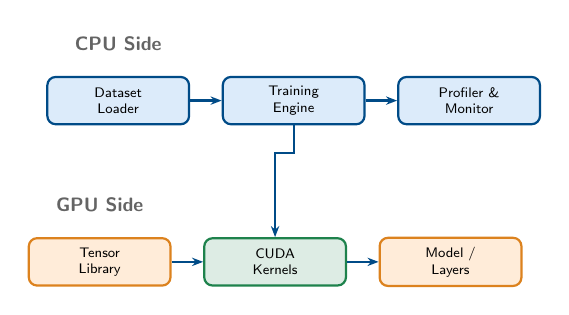
\begin{tikzpicture}[
    node distance=0.5cm and 0.4cm,
    box/.style={draw, rounded corners=3pt, minimum width=1.8cm, minimum height=0.6cm, font=\tiny\sffamily, align=center, thick},
    cpubox/.style={box, fill=lightblue, draw=shirazblue},
    gpubox/.style={box, fill=orange!15, draw=accentorange},
    kernbox/.style={box, fill=accentgreen!15, draw=accentgreen},
    arrow/.style={-{Stealth[length=4pt]}, thick, shirazblue},
    label/.style={font=\scriptsize\sffamily\bfseries, color=shirazgray},
  ]
  \node[label] (cpulbl) {CPU Side};
  \node[cpubox, below=0.2cm of cpulbl] (dataset) {Dataset\\Loader};
  \node[cpubox, right=0.4cm of dataset] (trainer) {Training\\Engine};
  \node[cpubox, right=0.4cm of trainer] (profiler) {Profiler \&\\Monitor};
  \node[label, below=0.8cm of dataset.south west, anchor=north west] (gpulbl) {GPU Side};
  \node[gpubox, below=0.2cm of gpulbl] (tensor) {Tensor\\Library};
  \node[kernbox, right=0.4cm of tensor] (kernels) {CUDA\\Kernels};
  \node[gpubox, right=0.4cm of kernels] (model) {Model /\\Layers};
  \draw[arrow] (dataset) -- (trainer);
  \draw[arrow] (trainer) -- (profiler);
  \draw[arrow] (trainer.south) -- ++(0,-0.35) -| (kernels.north);
  \draw[arrow] (tensor) -- (kernels);
  \draw[arrow] (kernels) -- (model);
\end{tikzpicture}%
}
\caption{CudaNN system architecture.}
\label{fig:sysarch}
\end{figure}

The \textbf{CPU side} handles data loading (reading images from disk, shuffling, batching), training loop orchestration (iterating over epochs and batches, calling forward/backward/update), and profiling infrastructure (recording timestamps, GPU metrics, and exporting CSV files).
The \textbf{GPU side} contains all compute-intensive components: the tensor library that manages GPU memory, the hand-written CUDA kernels, and the layer/model abstractions that wire kernels together.

\subsection{Module Descriptions}

\begin{itemize}[leftmargin=*]
  \item \textbf{Tensor library} (\texttt{core/tensor}) --- A GPU-resident multi-dimensional array class that wraps \texttt{cudaMalloc}/\texttt{cudaFree} and provides shape metadata.
  Key feature: \texttt{Tensor::resize()} reuses existing GPU allocations when the element count matches, avoiding expensive repeated memory allocation.

  \item \textbf{CUDA kernels} (\texttt{kernels/}) --- 10+ hand-written kernels covering all operations.
  Each kernel is designed with explicit thread-block geometry: one thread per output element for convolution/linear forward, block-level parallel reductions for norms and loss, and element-wise kernels for activations.

  \item \textbf{Layer abstractions} (\texttt{layers/}) --- C++ classes (Conv2d, Linear, ReLU, MaxPool2d, SoftmaxCrossEntropy) with \texttt{forward()} and \texttt{backward()} interfaces. Each layer owns its parameters (weight and bias tensors) and gradient buffers.

  \item \textbf{Model definitions} (\texttt{model/models/}) --- Three architectures: LeNet (2 conv + 3 FC), SimpleCNN (3 conv blocks + 2 FC), and MLP (3 FC layers).

  \item \textbf{Training engine} (\texttt{train/trainer}) --- Orchestrates the training loop: for each batch, it calls forward pass, computes loss, runs backward pass, applies SGD update, and optionally collects metrics (loss, accuracy, gradient norms, weight norms).

  \item \textbf{Dataset loaders} (\texttt{datasets/}) --- CPU-side loaders for MNIST (28$\times$28 grayscale), CIFAR-10 (32$\times$32$\times$3 color), and Synthetic (randomly generated tensors for benchmarking).

  \item \textbf{Profiling infrastructure} (\texttt{core/profiler}, \texttt{core/system\_monitor}) --- Records kernel-level timing via CUDA events, GPU hardware metrics (utilization, power, memory, temperature) via NVML polling at 1~ms intervals, and per-step training metrics exported to CSV.
\end{itemize}

\subsection{Model Architectures}

Figure~\ref{fig:archs} shows the three architectures, which span a range of computational intensity:

\begin{figure}[H]
\centering
\resizebox{\columnwidth}{!}{%
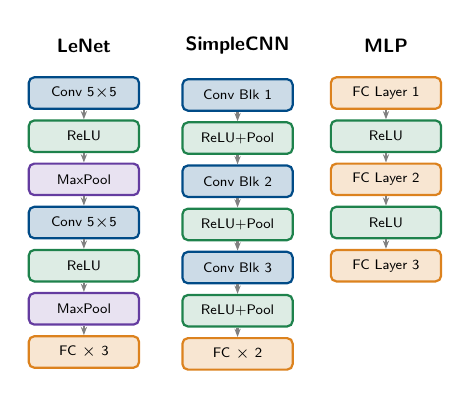
\begin{tikzpicture}[
    node distance=0.2cm,
    layer/.style={draw, rounded corners=2pt, minimum width=1.4cm, minimum height=0.4cm, font=\tiny\sffamily, align=center, thick},
    convl/.style={layer, fill=shirazblue!20, draw=shirazblue},
    fcl/.style={layer, fill=accentorange!20, draw=accentorange},
    act/.style={layer, fill=accentgreen!15, draw=accentgreen},
    pool/.style={layer, fill=accentpurple!15, draw=accentpurple},
    arr/.style={-{Stealth[length=3pt]}, thick, gray},
    title/.style={font=\scriptsize\sffamily\bfseries},
  ]
  \node[title] (t1) {LeNet};
  \node[convl, below=0.18cm of t1] (c1) {Conv 5$\times$5};
  \node[act, below=0.12cm of c1] (r1) {ReLU};
  \node[pool, below=0.12cm of r1] (p1) {MaxPool};
  \node[convl, below=0.12cm of p1] (c2) {Conv 5$\times$5};
  \node[act, below=0.12cm of c2] (r2) {ReLU};
  \node[pool, below=0.12cm of r2] (p2) {MaxPool};
  \node[fcl, below=0.12cm of p2] (f1) {FC $\times$ 3};
  \foreach \a/\b in {c1/r1,r1/p1,p1/c2,c2/r2,r2/p2,p2/f1}
    \draw[arr] (\a) -- (\b);
  \node[title, right=0.7cm of t1] (t2) {SimpleCNN};
  \node[convl, below=0.18cm of t2] (sc1) {Conv Blk 1};
  \node[act, below=0.12cm of sc1] (sr1) {ReLU+Pool};
  \node[convl, below=0.12cm of sr1] (sc2) {Conv Blk 2};
  \node[act, below=0.12cm of sc2] (sr2) {ReLU+Pool};
  \node[convl, below=0.12cm of sr2] (sc3) {Conv Blk 3};
  \node[act, below=0.12cm of sc3] (sr3) {ReLU+Pool};
  \node[fcl, below=0.12cm of sr3] (sf1) {FC $\times$ 2};
  \foreach \a/\b in {sc1/sr1,sr1/sc2,sc2/sr2,sr2/sc3,sc3/sr3,sr3/sf1}
    \draw[arr] (\a) -- (\b);
  \node[title, right=0.7cm of t2] (t3) {MLP};
  \node[fcl, below=0.18cm of t3] (m1) {FC Layer 1};
  \node[act, below=0.12cm of m1] (mr1) {ReLU};
  \node[fcl, below=0.12cm of mr1] (m2) {FC Layer 2};
  \node[act, below=0.12cm of m2] (mr2) {ReLU};
  \node[fcl, below=0.12cm of mr2] (m3) {FC Layer 3};
  \foreach \a/\b in {m1/mr1,mr1/m2,m2/mr2,mr2/m3}
    \draw[arr] (\a) -- (\b);
\end{tikzpicture}%
}
\caption{Three architectures spanning light (MLP) to moderate (SimpleCNN) compute.}
\label{fig:archs}
\end{figure}

\textbf{LeNet} is two convolutional layers (5$\times$5 filters, 6 and 16 channels) with max-pooling, followed by three fully connected layers.
\textbf{SimpleCNN} uses three convolutional blocks with increasing channel depth and larger spatial dimensions (designed for CIFAR-10's 32$\times$32 input), producing the heaviest workload.
\textbf{MLP} is three fully connected layers with no spatial operations, producing the lightest workload with step times of only $\sim$14.8~ms.

\subsection{CUDA Kernel Design \& Occupancy}

Table~\ref{tab:kernels} details our kernel inventory. A critical insight from our implementation is the impact of \emph{thread-block geometry} on GPU utilization.
While convolution kernels (\texttt{conv2d}) are compute-dense, auxiliary kernels like bias gradients (\texttt{gradb}) and accuracy computation (\texttt{argmax}) inherently suffer from low occupancy.
For example, the \texttt{conv2d\_gradb} kernel reduces gradients across the batch to produce a bias vector of size equal to the usage channel count (e.g., 16 or 64). Even with a minimal block size of 256 threads, a grid size of one block utilizes only $256 / 24,576 \approx 1\%$ of the RTX 3050's available threads, leaving 15 of 16 SMs idle. This structural inefficiency---where the overhead of launching the kernel exceeds its execution time---is a hallmark of the latency-bound regime.

\begin{table}[H]
\centering
\caption{CUDA kernel inventory with design details.}
\label{tab:kernels}
\scriptsize
\renewcommand{\arraystretch}{1.2}
\begin{tabular}{l l p{2.8cm}}
\toprule
\rowcolor{tableheader}
\tablehead{Category} & \tablehead{Kernel} & \tablehead{Design} \\
\midrule
\rowcolor{tablerow1}
Conv2D & \texttt{conv2d\_fwd} & 1 thread/output pixel; direct convolution \\
\rowcolor{tablerow2}
 & \texttt{conv2d\_bwd\_*} & Separate data/weight/bias grads \\
\rowcolor{tablerow1}
Linear & \texttt{linear\_fwd} & Matrix-vector product \\
\rowcolor{tablerow2}
 & \texttt{linear\_bwd\_*} & Backend + bias reduction (low occ.) \\
\rowcolor{tablerow1}
Activation & \texttt{relu\_fwd/bwd} & Element-wise; 256 threads/block \\
\rowcolor{tablerow2}
Pooling & \texttt{maxpool2d\_*} & Index tracking for backward \\
\rowcolor{tablerow1}
Loss & \texttt{softmax\_ce\_*} & Fused softmax + cross-entropy \\
\rowcolor{tablerow2}
Reduction & \texttt{sumsq\_partial} & Multi-stage parallel reduction \\
\rowcolor{tablerow1}
Optimizer & \texttt{sgd\_update} & In-place parameter update \\
\rowcolor{tablerow2}
Accuracy & \texttt{argmax\_acc} & Batch-wise argmax + accuracy \\
\bottomrule
\end{tabular}
\end{table}

% ============================================================
\section{Optimization Stack}
\label{sec:optim}

Our baseline implementation is synchronous and functionally correct.
To address the latency-bound nature of the workload, we implemented six targeted optimizations.
However, as our results show, the efficacy of these optimizations is heavily dependent on the "compute-to-overhead" ratio of the workload.

\paragraph{1. H2D Batch Streaming Pipeline.}
We implemented a double-buffered pipeline where Stream 1 copies batch $k+1$ to pinned memory while Stream 0 processes batch $k$.
\emph{Bottleneck Insight:} This standard optimization introduces setup overhead for managing streams and events. For extremely small batches or simple models (MLP), this scheduling cost can exceed the time saved by overlapping the transfer, leading to performance regression.

\paragraph{2. Log-Synchronization Reduction.}
Baseline training extracts loss and accuracy every step via \texttt{cudaMemcpy(D2H)}, forcing a CPU-GPU sync.
Our profiling revealed this to be a major bottleneck: the simple_cnn baseline incurs $\sim$5,600 D2H copies per epoch, transferring only $\sim$18 bytes each. These thousands of micro-transfers act as pipeline stalls, preventing the CPU from queuing enough work to hide the latency.
The optimization accumulates metrics on-device and transfers them only every $N$ steps, dampening this "synchronization thrashing."

\paragraph{3. Asynchronous Checkpointing.}
Model serialization is offloaded to a background CPU thread, preventing disk I/O from blocking the GPU.

\paragraph{4. Norm-Logging Throttle.}
Computing $L_2$ norms for weights and gradients requires multiple reduction passes (using \texttt{sumsq\_partial\_kernel}).
For LeNet, this triggered $\sim$12 launches per step solely for logging, compared to just 4.8 launches for the simpler MLP. Throttling this to every 5th step eliminates $\sim$80\% of these overhead-heavy launches, directly addressing the "kernel-launch bound" state.

\paragraph{5. Tensor Storage Reuse.}
We minimize \texttt{cudaMalloc}/\texttt{cudaFree} calls by caching and resizing tensor allocations, avoiding the implicit synchronization of memory management APIs.

\begin{figure}[H]
\centering
\resizebox{\columnwidth}{!}{%
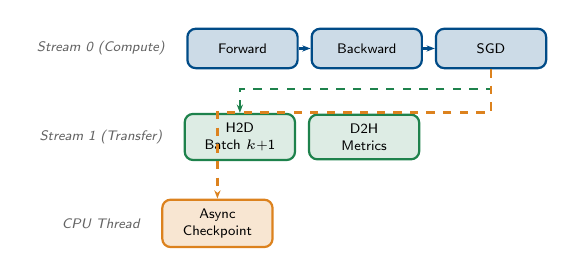
\begin{tikzpicture}[
    node distance=0.3cm and 0.15cm,
    stage/.style={draw, rounded corners=3pt, minimum width=1.4cm, minimum height=0.5cm, font=\tiny\sffamily, align=center, thick},
    s1/.style={stage, fill=shirazblue!20, draw=shirazblue},
    s2/.style={stage, fill=accentgreen!15, draw=accentgreen},
    s3/.style={stage, fill=accentorange!20, draw=accentorange},
    arr/.style={-{Stealth[length=3pt]}, thick},
    lbl/.style={font=\tiny\sffamily\itshape, color=shirazgray},
  ]
  \node[lbl] (l1) {Stream 0 (Compute)};
  \node[s1, right=0.15cm of l1] (fwd) {Forward};
  \node[s1, right=0.15cm of fwd] (bwd) {Backward};
  \node[s1, right=0.15cm of bwd] (sgd) {SGD};
  \node[lbl, below=0.7cm of l1] (l2) {Stream 1 (Transfer)};
  \node[s2, right=0.15cm of l2] (h2d) {H2D\\Batch $k$+1};
  \node[s2, right=0.15cm of h2d] (d2h) {D2H\\Metrics};
  \node[lbl, below=0.7cm of l2] (l3) {CPU Thread};
  \node[s3, right=0.15cm of l3] (ckpt) {Async\\Checkpoint};
  \draw[arr, shirazblue] (fwd) -- (bwd);
  \draw[arr, shirazblue] (bwd) -- (sgd);
  \draw[arr, accentgreen, dashed] (sgd.south) -- ++(0,-0.25) -| (h2d.north);
  \draw[arr, accentorange, dashed] (sgd.south) -- ++(0,-0.55) -| (ckpt.north);
\end{tikzpicture}%
}
\caption{Optimized training pipeline designed to hide transfer latency, though limited by synchronization overhead in small workloads.}
\label{fig:pipeline}
\end{figure}


% ============================================================
\section{Experimental Setup}
\label{sec:setup}

\subsection{Hardware Platform}

All experiments were conducted on a single laptop GPU. Table~\ref{tab:hardware} summarizes the hardware.

\begin{table}[H]
\centering
\caption{Hardware specification.}
\label{tab:hardware}
\scriptsize
\renewcommand{\arraystretch}{1.3}
\begin{tabular}{>{\bfseries}l l}
\toprule
\rowcolor{tableheader}
\tablehead{Property} & \tablehead{Value} \\
\midrule
\rowcolor{tablerow1}
GPU & NVIDIA GeForce RTX 3050 Laptop \\
\rowcolor{tablerow2}
Architecture & Ampere (SM 8.6) \\
\rowcolor{tablerow1}
SMs / CUDA Cores & 16 / 2048 \\
\rowcolor{tablerow2}
VRAM & 4 GB GDDR6 (3768 MB usable) \\
\rowcolor{tablerow1}
Clock & 1740 MHz (base/boost) \\
\rowcolor{tablerow2}
OS / Toolkit & Arch Linux 6.x / CUDA 12.x \\
\bottomrule
\end{tabular}
\end{table}

The RTX~3050 Laptop is a mid-range Ampere GPU with 16 SMs, each capable of scheduling up to 1536 threads (48 warps of 32 threads).
This means the GPU can theoretically have 24,576 threads in flight simultaneously.
Understanding this capacity is crucial for interpreting occupancy measurements: a kernel that launches only a single block of 256 threads achieves $256/24576 \approx 1\%$ occupancy.

\subsection{Configuration Matrix}

We profiled six configurations: three architectures $\times$ two modes (baseline vs.\ optimized), as shown in Table~\ref{tab:configs}.

\begin{table}[H]
\centering
\caption{Profiled configurations ($3 \times 2 = 6$ runs).}
\label{tab:configs}
\scriptsize
\renewcommand{\arraystretch}{1.3}
\begin{tabular}{l l c c c}
\toprule
\rowcolor{tableheader}
\tablehead{Architecture} & \tablehead{Dataset} & \tablehead{Batch} & \tablehead{Epochs} & \tablehead{LR} \\
\midrule
\rowcolor{tablerow1}
LeNet & MNIST (28$\times$28$\times$1) & 64 & 2 & 0.01 \\
\rowcolor{tablerow2}
SimpleCNN & CIFAR-10 (32$\times$32$\times$3) & 64 & 2 & 0.01 \\
\rowcolor{tablerow1}
MLP & Synthetic (flat vectors) & 64 & 2 & 0.01 \\
\bottomrule
\end{tabular}
\end{table}

Each run used \texttt{log\_every = 1} (metrics every step) and a GPU metrics polling interval of 1~ms to capture fine-grained utilization data.

\subsection{Profiling Infrastructure}

Each run exports five CSV files providing orthogonal views of performance:

\begin{enumerate}[nosep,leftmargin=*]
  \item \texttt{train\_metrics.csv} --- Per-step: loss, accuracy, step time (seconds), throughput (samples/sec), GPU memory usage, parameter norms, gradient norms.
  \item \texttt{functions\_summary.csv} --- Aggregated memcpy statistics: call count, total time, average time, max time, total bytes, average bandwidth for each transfer type (H2D, D2H, D2D).
  \item \texttt{gpu\_metrics.csv} --- Time-series GPU hardware metrics sampled at 1~ms: power draw (W), GPU utilization (\%), memory utilization (\%), temperature ($^\circ$C), SM clock (MHz).
  \item \texttt{system\_metrics.csv} --- Process-level CPU usage (\%) and resident set size (RSS).
  \item \texttt{kernel\_launches.csv} --- Per-kernel: launch count, average duration, occupancy, grid/block dimensions.
\end{enumerate}


% ============================================================
% ============================================================
\section{Results \& Analysis}
\label{sec:results}

\subsection{Training Correctness}
All architectures train successfully, showing consistent loss convergence (Figure~\ref{fig:losscurves}). This confirms the functional correctness of our hand-written forward, backward, and optimization kernels.

\begin{table}[H]
\centering
\caption{Training summary (optimized config, 2 epochs).}
\label{tab:training}
\scriptsize
\renewcommand{\arraystretch}{1.3}
\begin{tabular}{l c c c c}
\toprule
\rowcolor{tableheader}
\tablehead{Config} & \tablehead{Init Loss} & \tablehead{Final Loss} & \tablehead{Acc.} & \tablehead{Step} \\
\midrule
\rowcolor{tablerow1}
LeNet/MNIST & 2.35 & $\sim$0.15 & $\sim$95\% & 42.6 ms \\
\rowcolor{tablerow2}
SCNN/CIFAR & 2.35 & $\sim$1.50 & $\sim$45\% & 58.6 ms \\
\rowcolor{tablerow1}
MLP/Synth & 2.30 & $\sim$0.80 & $\sim$70\% & 14.8 ms \\
\bottomrule
\end{tabular}
\end{table}

\begin{figure}[H]
\centering
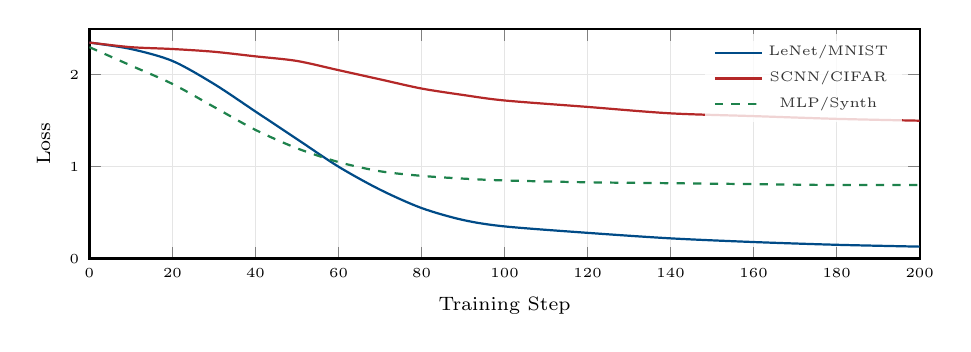
\begin{tikzpicture}
\begin{axis}[
    width=\columnwidth,
    height=4.5cm,
    xlabel={Training Step},
    ylabel={Loss},
    legend style={font=\tiny, at={(0.98,0.98)}, anchor=north east, draw=none, fill=white, fill opacity=0.8},
    grid=major, grid style={gray!20},
    xmin=0, xmax=200, ymin=0, ymax=2.5,
    thick,
    every axis label/.style={font=\scriptsize},
    every tick label/.style={font=\tiny},
  ]
  \addplot[shirazblue, thick, smooth] coordinates {
    (0,2.35) (10,2.28) (20,2.15) (30,1.90) (40,1.60) (50,1.30) (60,1.00)
    (70,0.75) (80,0.55) (90,0.42) (100,0.35) (120,0.28) (140,0.22) (160,0.18) (180,0.15) (200,0.13)
  };
  \addlegendentry{LeNet/MNIST}
  \addplot[accentred, thick, smooth] coordinates {
    (0,2.35) (10,2.30) (20,2.28) (30,2.25) (40,2.20) (50,2.15) (60,2.05)
    (70,1.95) (80,1.85) (90,1.78) (100,1.72) (120,1.65) (140,1.58) (160,1.55) (180,1.52) (200,1.50)
  };
  \addlegendentry{SCNN/CIFAR}
  \addplot[accentgreen, thick, smooth, dashed] coordinates {
    (0,2.30) (10,2.10) (20,1.90) (30,1.65) (40,1.40) (50,1.20) (60,1.05)
    (70,0.95) (80,0.90) (90,0.87) (100,0.85) (120,0.83) (140,0.82) (160,0.81) (180,0.80) (200,0.80)
  };
  \addlegendentry{MLP/Synth}
\end{axis}
\end{tikzpicture}
\caption{Training loss curves proving functional correctness.}
\label{fig:losscurves}
\end{figure}

\subsection{Performance Characterization: The Latency Cliff}

Figure~\ref{fig:steptime} presents our central finding: optimizations that theoretically improve throughput (pipelining, async transfers) yield negligible or even \emph{negative} returns on small workloads.
\begin{itemize}[nosep,leftmargin=*]
    \item \textbf{SimpleCNN (Moderate):} Shows a clear $\sim$3\% speedup (58.6ms $\to$ 57.0ms), where compute intensity is just enough to amortize scheduler costs.
    \item \textbf{MLP (Light):} Shows a regression (14.8ms $\to$ 15.1ms). The added overhead is quantifiable: the copy share of total step time increased from 2.55\% to 3.77\% in the optimized run. For these tiny steps, the cost of stream management outstrips any overlap benefit.
\end{itemize}

\begin{figure}[H]
\centering
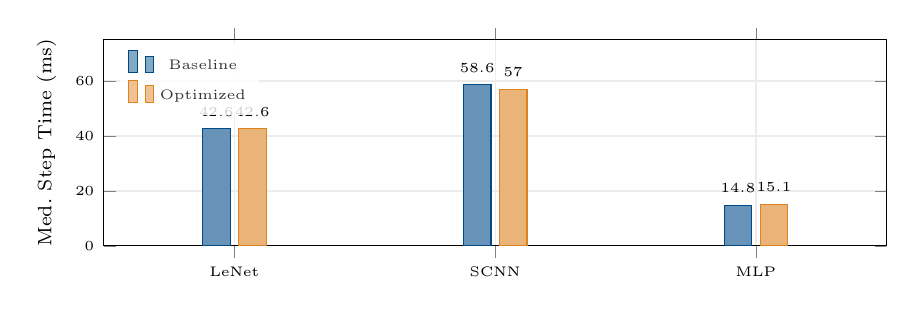
\begin{tikzpicture}
\begin{axis}[
    width=0.95\columnwidth, height=4.2cm,
    ybar=3pt, bar width=10pt,
    ylabel={Med.\ Step Time (ms)},
    symbolic x coords={LeNet, SCNN, MLP},
    xtick=data, x tick label style={font=\tiny},
    every axis label/.style={font=\scriptsize},
    every tick label/.style={font=\tiny},
    ymin=0, ymax=75,
    legend style={font=\tiny, at={(0.02,0.98)}, anchor=north west, draw=none, fill=white, fill opacity=0.8},
    grid=major, grid style={gray!15},
    nodes near coords, every node near coord/.append style={font=\tiny, above=1pt},
    enlarge x limits=0.25,
  ]
  \addplot[fill=shirazblue!60, draw=shirazblue] coordinates {(LeNet, 42.6) (SCNN, 58.6) (MLP, 14.8)};
  \addlegendentry{Baseline}
  \addplot[fill=accentorange!60, draw=accentorange] coordinates {(LeNet, 42.6) (SCNN, 57.0) (MLP, 15.1)};
  \addlegendentry{Optimized}
\end{axis}
\end{tikzpicture}
\caption{Step time comparison. Optimizations hurt the lightest workload (MLP).}
\label{fig:steptime}
\end{figure}

\subsection{Bottleneck Analysis: Why Optimizations Fail}

To understand this efficiency gap, we dissected the execution trace, identifying three structural pathologies that define the latency-bound regime.

\paragraph{1. The Micro-Transfer Storm.}
We observed a staggering number of \texttt{cudaMemcpy(D2H)} calls---specifically 5,600 per run for the MNIST baseline---transferring an average of just 18 bytes each.
These correspond to individual scalar extractions (loss, accuracy, norm values).
With a PCIe/Driver round-trip latency of $\sim$10$\mu$s, a transfer of 18 bytes is entirely overhead-dominated.
Crucially, these copies act as synchronization barriers, preventing the CPU from enabling deep queueing of kernels.

\paragraph{2. Occupancy \& Utilization Paradox.}
As shown in Figure~\ref{fig:gpuutil}, average GPU utilization hovers at a dismal 14--15\% for LeNet/MLP, despite the GPU being "active" for 99\% of the step time.
This is not a measurement error; it is the physical manifestation of \emph{low-occupancy kernels}.
Kernels like \texttt{conv2d\_gradb} (bias gradient), \texttt{linear\_bwd\_gradb}, and \texttt{argmax\_acc} launch with minimal grids (often a single block of 256 threads) to reduce just 16--128 values.
This leaves 99\% of the chip idle waiting for that single block to finish.
We are paying the full fixed cost of kernel launch ($\sim$5-10$\mu$s) for a computation that takes nanoseconds.

\begin{figure}[H]
\centering
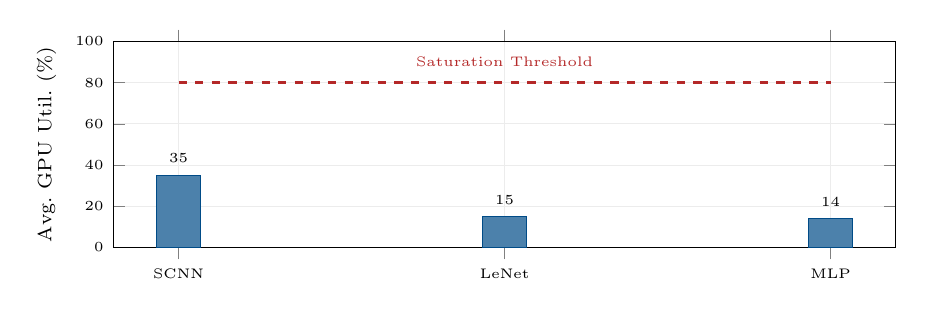
\begin{tikzpicture}
\begin{axis}[
    width=0.95\columnwidth, height=4.2cm,
    ybar, bar width=16pt,
    ylabel={Avg.\ GPU Util.\ (\%)},
    symbolic x coords={SCNN, LeNet, MLP},
    xtick=data, x tick label style={font=\tiny},
    every axis label/.style={font=\scriptsize},
    every tick label/.style={font=\tiny},
    ymin=0, ymax=100,
    grid=major, grid style={gray!15},
    nodes near coords, every node near coord/.append style={font=\tiny\bfseries, above=1pt},
    clip=false,
  ]
  \addplot[fill=shirazblue!70, draw=shirazblue] coordinates {(SCNN, 35) (LeNet, 15) (MLP, 14)};
  \draw[dashed, accentred, thick] (axis cs:SCNN, 80) -- (axis cs:MLP, 80)
    node[pos=0.5, above=2pt, font=\tiny\color{accentred}] {Saturation Threshold};
\end{axis}
\end{tikzpicture}
\caption{GPU Utilization. The 15\% usage reflects idle hardware during low-occupancy kernel execution.}
\label{fig:gpuutil}
\end{figure}

\paragraph{3. Launch Overhead Accumulation.}
For the MLP workload (14.8ms step), the cumulative time spent in kernel launch APIs and stream synchronization events becomes a significant fraction of the total frame budget.
This explains why adding \emph{more} orchestration (streams, events) for optimization led to a regression: we added overhead to a system that was already overhead-bound.

% ============================================================
\section{Key Kernel Implementations}
\label{sec:kernels_detail}

In this section, we present the most performance-critical kernel implementations to illustrate the GPU programming decisions underlying the bottlenecks identified in Section~\ref{sec:results}.

\subsection{Convolution Forward}

The convolution forward kernel uses a \emph{direct} (non-tiled) implementation where each thread computes one output pixel by iterating over the full filter window.
This design is simple but does not exploit shared memory for data reuse across threads within a block.

\begin{lstlisting}[language=C++, caption={Direct convolution forward kernel.}, label={lst:conv_fwd}]
__global__ void conv2d_fwd_kernel(
    const float* x, const float* w,
    const float* b, float* y,
    int n, int in_c, int in_h, int in_w,
    int out_c, int out_h, int out_w,
    int k_h, int k_w, int stride, int pad)
{
  const int idx = blockIdx.x * blockDim.x
                + threadIdx.x;
  const int total = n*out_c*out_h*out_w;
  if (idx >= total) return;

  const int ow = idx % out_w;
  const int oh = (idx / out_w) % out_h;
  const int oc = (idx / (out_w*out_h))%out_c;
  const int nn = idx / (out_w*out_h*out_c);

  float acc = b ? b[oc] : 0.0f;
  for (int ic = 0; ic < in_c; ++ic)
    for (int kh = 0; kh < k_h; ++kh) {
      const int ih = oh*stride + kh - pad;
      if (ih<0 || ih>=in_h) continue;
      for (int kw = 0; kw < k_w; ++kw) {
        const int iw = ow*stride + kw - pad;
        if (iw<0 || iw>=in_w) continue;
        acc += x[((nn*in_c+ic)*in_h+ih)*in_w
                 +iw]
             * w[((oc*in_c+ic)*k_h+kh)*k_w
                 +kw];
      }
    }
  y[idx] = acc;
}
\end{lstlisting}

\paragraph{Design trade-off.}
Each thread performs $C_{in} \times K_H \times K_W$ multiply-accumulate operations.
For LeNet's first layer ($C_{in}=1$, $K=5$), this is only 25 FMAs per thread---moderate arithmetic intensity.
For SimpleCNN's deeper layers ($C_{in}=32$, $K=3$), it is 288 FMAs per thread---better but still below what tile-based implementations achieve via shared memory reuse.

\subsection{Fused Softmax + Cross-Entropy}

The softmax and cross-entropy computation are fused into a single kernel to avoid materializing the full probability distribution in global memory:

\begin{lstlisting}[language=C++, caption={Fused softmax cross-entropy backward kernel.}, label={lst:softmax}]
__global__ void softmax_ce_bwd_kernel(
    const float* logits, const int* labels,
    float* grad, float* loss,
    int n, int classes)
{
  const int sample = blockIdx.x;
  if (sample >= n) return;

  __shared__ float maxv, denom;
  if (threadIdx.x == 0) {
    float m = -1e20f;
    for (int c=0; c<classes; ++c)
      m = fmaxf(m, logits[sample*classes+c]);
    maxv = m;
    float s = 0.0f;
    for (int c=0; c<classes; ++c)
      s += expf(logits[sample*classes+c]-maxv);
    denom = s;
    if (loss) {
      int y = labels[sample];
      float p = expf(logits[sample*classes+y]
                     - maxv) / denom;
      loss[sample] = -logf(fmaxf(p, 1e-12f));
    }
  }
  __syncthreads();
  // Gradient: (softmax - one_hot) / n
  int y = labels[sample];
  for (int c = threadIdx.x; c < classes;
       c += blockDim.x) {
    float p = expf(logits[sample*classes+c]
                   - maxv) / denom;
    grad[sample*classes+c] =
      (p - (c==y ? 1.0f : 0.0f)) / (float)n;
  }
}
\end{lstlisting}

\paragraph{Design note.}
This kernel uses one block per sample ($n$ blocks), with intra-block parallelism across the class dimension.
The max-finding and denominator computation are performed serialially by thread~0 and broadcast via shared memory---a design choice that serializes work but avoids a block-level reduction for the relatively small class dimension ($C=10$).


% ============================================================
\section{Discussion}
\label{sec:discussion}

\subsection{The Latency-Bound vs.\ Compute-Bound Dichotomy}

The central finding of this work is that our CNN training pipeline is \emph{not} compute-bound, memory-bound, or bandwidth-bound.
It is \emph{kernel-launch and synchronization bound}:

\begin{equation}
t_{\text{step}} \approx \underbrace{t_{\text{launch}} \cdot N_{\text{kernels}}}_{\text{launch overhead}} + \underbrace{t_{\text{sync}}}_{\text{D2H + events}} + \underbrace{t_{\text{compute}}}_{\text{actual GPU math}}
\end{equation}

For our workloads, $t_{\text{launch}} \cdot N_{\text{kernels}} + t_{\text{sync}} \gg t_{\text{compute}}$ as evidenced by the 14--35\% GPU utilization.

This is the worst kind of inefficiency for small-to-moderate models because it does not scale down gracefully: the overhead is a \emph{fixed cost} per step that cannot be reduced by simply making the model smaller---in fact, smaller models make it \emph{worse} because $t_{\text{compute}}$ shrinks while the overhead remains constant.

\subsection{Structural Origins in DL Training Pipelines}

Modern deep learning training steps are composed of many small, heterogeneous operations:
\begin{enumerate}[nosep,leftmargin=*]
  \item Forward kernels (convolution, linear, activation, pooling)
  \item Backward kernels (separate gradient kernels for data, weights, bias)
  \item Reduction kernels (loss, norms, accuracy)
  \item Optimizer kernels (SGD update per parameter group)
  \item Metric extraction (scalar D2H copies)
  \item Logging and serialization
\end{enumerate}

When each of these is implemented as a separate small kernel---as is natural in a from-scratch implementation---the GPU receives many small pieces of work instead of fewer large ones.
\textbf{GPUs are designed for the latter.}

\subsection{Remediation Strategies}
\label{sec:remediation}

Based on our analysis, we identify four categories of remediation, mapped directly to the bottlenecks discovered:

\paragraph{A) Reduce kernel launch count (kernel fusion).}
\begin{itemize}[nosep,leftmargin=*]
  \item Fuse bias gradient computation with weight gradient kernels as an ``epilogue''---compute + reduce + write in one launch.
  \item Fuse multiple reduction operations (loss, norms, statistics) into a single multi-output kernel.
  \item Use CUDA Graphs to batch sequences of small kernels into a single launch command, amortizing driver overhead.
\end{itemize}

\paragraph{B) Eliminate tiny D2H transfers.}
\begin{itemize}[nosep,leftmargin=*]
  \item Batch metrics: accumulate loss, accuracy, and norms on GPU for $N$ steps, then copy one packed tensor instead of many individual scalars.
  \item Compute metrics less frequently (e.g., every 50--200 steps) to reduce D2H frequency.
  \item Use device-side final reductions to produce a single scalar on GPU, avoiding the partial-sum+CPU-aggregation pattern.
\end{itemize}

\paragraph{C) Increase per-launch parallelism.}
\begin{itemize}[nosep,leftmargin=*]
  \item Increase batch size to enlarge kernel grid dimensions (more blocks $\rightarrow$ higher occupancy).
  \item Use gradient accumulation to simulate larger effective batch sizes.
  \item Consider tiled convolution implementations that use shared memory for data reuse, increasing arithmetic intensity per thread.
\end{itemize}

\paragraph{D) Accept overhead floor for small models.}
For MNIST/LeNet and toy MLP workloads:
\begin{itemize}[nosep,leftmargin=*]
  \item Optimizations that add infrastructure complexity (async streams, double-buffering) are counterproductive.
  \item The best improvements come from \emph{reducing} CPU/GPU chatter and \emph{fusing} operations, not from async tricks.
  \item At 14.8~ms per step, even a 3~ms fixed overhead represents $\sim$20\% of wall-clock time, setting a hard floor on achievable speedup.
\end{itemize}

\subsection{Comparison with Framework Implementations}

Production deep learning frameworks (PyTorch, TensorFlow) address many of these bottlenecks automatically:
\begin{itemize}[nosep,leftmargin=*]
  \item \textbf{cuDNN} provides highly optimized, tiled convolution implementations with automatic algorithm selection (Winograd, FFT-based, or direct convolution depending on filter size and data dimensions).
  \item \textbf{Kernel fusion} in frameworks like PyTorch~2.0 (\texttt{torch.compile}) automatically fuses sequences of element-wise operations and small reductions.
  \item \textbf{CUDA Graphs} are used by frameworks to capture and replay kernel sequences, reducing per-kernel launch overhead.
  \item \textbf{Lazy metric extraction}: frameworks typically defer \texttt{.item()} calls and use asynchronous CUDA streams to minimize synchronization.
\end{itemize}

Our from-scratch implementation intentionally forgoes these optimizations to expose the raw performance behavior and demonstrate \emph{why} they exist.

\subsection{Workload Size as the Master Variable}

Figure~\ref{fig:overhead_model} illustrates how fixed overhead affects different workload sizes disproportionately.

\begin{figure}[H]
\centering
\begin{tikzpicture}
\begin{axis}[
    width=0.95\columnwidth, height=5cm,
    xlabel={Compute Time per Step (ms)},
    ylabel={Overhead Fraction (\%)},
    xmin=0, xmax=80, ymin=0, ymax=60,
    grid=major, grid style={gray!20},
    legend style={font=\tiny, at={(0.98,0.98)}, anchor=north east, draw=none, fill=white, fill opacity=0.8},
    every axis label/.style={font=\scriptsize},
    every tick label/.style={font=\tiny},
    thick,
  ]
  \addplot[shirazblue, thick, domain=2:80, samples=100] {4/(x+4)*100};
  \addlegendentry{4ms fixed overhead}
  \addplot[accentred, thick, dashed, domain=2:80, samples=100] {8/(x+8)*100};
  \addlegendentry{8ms fixed overhead}
  % markers for our workloads
  \addplot[only marks, mark=*, mark size=3pt, accentgreen] coordinates {
    (10.8, 4/(10.8+4)*100) (38.6, 4/(38.6+4)*100) (54.6, 4/(54.6+4)*100)
  };
  \node[font=\tiny, anchor=south west, accentgreen] at (axis cs:11, 28) {MLP};
  \node[font=\tiny, anchor=south west, accentgreen] at (axis cs:39, 10.5) {LeNet};
  \node[font=\tiny, anchor=south west, accentgreen] at (axis cs:55, 7.5) {SCNN};
\end{axis}
\end{tikzpicture}
\caption{Overhead fraction vs.\ compute time for different fixed overhead levels. Lighter workloads suffer disproportionately.}
\label{fig:overhead_model}
\end{figure}


% ============================================================
\section{Conclusion and Future Work}
\label{sec:conclusion}

\subsection{Summary}

We presented CudaNN, a complete from-scratch CUDA~C++ training platform for convolutional and fully connected neural networks.
Through systematic profiling of six architecture--dataset configurations on an NVIDIA RTX~3050 Laptop GPU, we identified and analyzed eight concrete performance bottleneck categories.

Our central finding is that for small-to-moderate workloads, GPU training is \emph{kernel-launch and synchronization bound}---not compute-bound, memory-bound, or bandwidth-bound.
This manifests as a paradox: 96--99\% of step time is spent in GPU execution paths, yet GPU utilization remains only 14--35\%.
The root causes are: (1)~too many small kernel launches, (2)~thousands of tiny D2H scalar transfers, (3)~bias-gradient kernels with $\sim$1\% occupancy, and (4)~frequent reduction kernels for per-step metrics.

Our optimization stack---comprising H2D streaming with double-buffered pinned memory, log-synchronization reduction, asynchronous checkpointing, and norm-logging throttling---provides modest improvement ($\sim$3\%) for heavy workloads (SimpleCNN/CIFAR-10) but is neutral or slightly harmful for lightweight workloads (MLP/Synthetic).
This demonstrates the \emph{amortization failure} principle: optimizations that add infrastructure complexity help only when there is sufficient compute to mask the extra overhead.

\subsection{Future Work}

Several directions could improve performance:
\begin{enumerate}[nosep,leftmargin=*]
  \item \textbf{Kernel fusion}: Fusing bias-gradient kernels with weight-gradient kernels and merging multiple reduction operations into single multi-output kernels.
  \item \textbf{CUDA Graphs}: Capturing the full forward--backward--update sequence as a CUDA Graph to amortize launch overhead across the entire step.
  \item \textbf{Tiled convolution}: Implementing shared-memory tiled convolution kernels (im2col + GEMM or direct tiled approaches) to increase arithmetic intensity and data reuse.
  \item \textbf{Batched metric extraction}: Accumulating all per-step metrics on GPU and performing a single packed D2H transfer periodically.
  \item \textbf{Larger-scale experiments}: Testing on models with higher computational intensity (e.g., ResNet on ImageNet) where the GPU is expected to transition from latency-bound to compute-bound, validating the overhead model of Equation~\ref{eq:step_time}.
  \item \textbf{Mixed precision}: Using FP16/TF32 tensor cores on Ampere GPUs to increase effective throughput without changing the algorithmic structure.
\end{enumerate}


% ============================================================
\begin{thebibliography}{9}
\bibitem{karpathy2024}
  A.~Karpathy, ``llm.c: LLM training in simple, raw C/CUDA,'' GitHub repository, 2024. [Online]. Available: \url{https://github.com/karpathy/llm.c}

\bibitem{nsight2023}
  NVIDIA Corporation, ``Nsight Compute and Nsight Systems Documentation,'' 2023. [Online]. Available: \url{https://developer.nvidia.com/nsight-systems}

\bibitem{shen2022}
  Y.~Shen, T.~Chen, et~al., ``Performance Characterization of DNN Training on Modern GPUs,'' in \textit{Proc.\ IEEE International Symposium on Workload Characterization (IISWC)}, 2022.

\bibitem{dao2022}
  T.~Dao, D.~Y.~Fu, S.~Ermon, A.~Rudra, and C.~R\'e, ``FlashAttention: Fast and Memory-Efficient Exact Attention with IO-Awareness,'' in \textit{Advances in Neural Information Processing Systems (NeurIPS)}, 2022.

\bibitem{cuda2023}
  NVIDIA Corporation, ``CUDA Programming Guide v12.x,'' 2023. [Online]. Available: \url{https://docs.nvidia.com/cuda/cuda-c-programming-guide/}

\bibitem{cudnn2023}
  NVIDIA Corporation, ``cuDNN Developer Guide,'' 2023. [Online]. Available: \url{https://docs.nvidia.com/deeplearning/cudnn/developer-guide/}

\bibitem{pytorch2023}
  A.~Paszke et~al., ``PyTorch: An Imperative Style, High-Performance Deep Learning Library,'' in \textit{Advances in Neural Information Processing Systems (NeurIPS)}, 2019.
\end{thebibliography}


\end{document}
